\chapter{Symmetrien der Geradenkonfiguration} \label{chap:configsymm}
\section{Lineare und Kombinatorische Symmetrien}
Die Fermat-Flächen haben einen hohen Grad an Symmetrie. Offenbar lassen sowohl Permutationen der Koordinaten als auch Multiplikation der Koordinaten mit $d$-ten Einheitswurzeln die Fläche invariant. Damit operieren die Gruppen $S_4$ und $\mu_d^4$, letztere mit Stabilisator \note Heißt das so? isomorph zu $\mu_d$. Beide Gruppen schneiden sich nur in $\{\id\}$, also haben wir eine Aktion von
\begin{equation}
S_4 \ltimes \mu_d^4 / \mu_d \subset \PGL 4K,
\end{equation}
auf $F_d$, wobei der Homomorphismus $S_4 \rightarrow \Aut(\mu_d^4 / \mu_d)$ auf Permutationen der Koordinaten abbildet. In bestimmten Fällen gibt es sogar noch mehr Symmetrien, wie wir später sehen werden. Allgemein interessieren wir uns für Abbildungen aus~$\PGL 4K$ bzw.~$\PGaL 4K$, die die Fläche $F_d$ invariant lassen.\footnote{Für eine Theorie der linearen Gruppen, speziell der $\PGaL nK$, siehe \cite{Dieudonne}.}
\begin{defin}
Sei $S \in \proj n(K)$ eine beliebige Menge. Als lineare Symmetriegruppe von $S$ bezeichnen wir die Untergruppe
\begin{equation}
G_l = G_l(S) = \{ g \in \PGL{n+1}K: gS = S \}.
\end{equation}
\end{defin}

Solche linearen Abbildungen lassen nicht nur die Fläche invariant, sondern schicken auch Geraden auf Geraden. Damit permutieren sie die Geraden auf der Fläche, offenbar bleibt dabei aber ihre Schnittkonfiguration erhalten. Die Schnittkonfiguration wird durch einen Graphen $\mathcal G = (L,E)$ kodiert, dabei ist die $L$ die Menge der Geraden, und $(l_1, l_2) \in E$, wenn $l_1$ und $l_2$ sich schneiden.

Die Frage liegt nahe, welche Permutationen der Geraden es denn gibt, die die Schnittkonfiguration erhalten.
\begin{defin}
Sei nun $S \in \proj 3(K)$ eine projektive Fläche, $\mathcal G = (L,E)$ die Geradenkonfiguration. Dann ist die kombinatorische Symmetriegruppe von $S$ die Automorphismengruppe des Graphen $\mathcal G$, d.h.
\begin{equation}
G_k = G_k(S) = \{ \sigma \in \Sym(L): (l_1, l_2) \in E \Leftrightarrow (\sigma(l_1), \sigma(l_2)) \in E \}
\end{equation}
\end{defin}
Wir wollen in diesem Kapitel die Beziehung zwischen diesen beiden Gruppen ausarbeiten. Die folgende Betrachtung ist inspiriert durch \cite[Bem.~4.10.1, S.~404]{Hartshorne}, und \cite[Aufg. C--D, S.~180]{Mumford}. Dort wird die Situation für allgemeine reguläre Flächen dritten Grades untersucht.

Wie oben bemerkt, induziert jede lineare Symmetrie eine kombinatorische, also haben wir einen Homomorphismus $G_l(F_d) \to G_k(F_d)$.
\begin{prop}
Gibt es unter den Schnittpunkten der Geraden auf $S$ mindestens fünf in allgemeiner Lage,\footnote{das heißt: keine vier davon liegen auf einer projektiven Ebene.} so ist der Homomorphismus $G_l(S) \to G_k(S)$ injektiv.
\end{prop}
\begin{proof}
Sei $g \in \PGL 4K$ so gewählt, dass alle Geraden auf $S$ auf sich selbst abgebildet werden. Dann werden auch vier der Schnittpunkte auf sich selbst abgebildet. Sei $A \in \GL 4K$ ein Urbild von $g$, dann lässt also $A$ vier linear unabhängige eindimensionale Teilräume in $K^4$ invariant. Folglich hat $A$ in einer geeigneten Basis ${v_1, \dots v_4}$ des $K^4$ als Matrix Diagonalgestalt.

Sei $v_5 \in K^4 \setminus 0$ ein zugehöriger Vektor zum fünften Schnittpunkt. In der Basis $\{v_i\}_{i<5}$ hat $v_5$ dann die Gestalt $\sum_i \alpha_i v_i$ mit $\alpha_i \neq 0$ für alle $i$, da die fünf Schnittpunkte in allgemeiner Lage sind. Weil der fünfte Punkt von $g$ auf sich selbst geschickt wird, ist $A v_5 = \lambda v_5$ für ein $\lambda \in K^*$. Damit sind die Diagonaleinträge der Matrix alle gleich $\lambda$, da die $\alpha_i$ nicht verschwinden. Also ist $A = \lambda \id$ bzw.~$g = \id$.
\end{proof}
Wie wir weiter unten sehen werden, schneiden sich zwei Geraden einer Klasse in Punkten der Form $(1:\zeta^n:0:0)$, $\zeta \in \mu_{2d}$ primitiv und $n$ ungerade; sowie Permutationen der Koordinaten. Durch Probieren findet man damit leicht fünf Punkte in allgemeiner Lage. Die fünf $4 \times 4$-Untermatrizen von
\begin{equation*}
\begin{pmatrix}
1 & 0 & 1 & 0 & 1 \\
\zeta & 0 & 0 & 1 & 0 \\
0 & 1 & \zeta^3 & 0 & 0 \\
0 & \zeta & 0 & \zeta^5 & \zeta^3 \\
\end{pmatrix}
\end{equation*}
haben Determinanten $(\zeta^2-1)\zeta^4$, $(\zeta+1)\zeta^4$, $-(\zeta^3+1)\zeta^3$, $-(\zeta^3+1)\zeta^6$ bzw.~$(\zeta+1)\zeta^3$. Für $d>3$ verschwindet keine davon.

\section{Reguläre Geraden}
\paragraph{Konfiguration} Wir schreiben die Geraden aus \eqref{eq:regular} mit einer fixierten primitiven Einheitswurzel $\zeta \in \mu_{2d}$ und $a,b \in (2\mathbb Z + 1)/2d\mathbb Z \subset \Zmod 2dZ$:
\begin{equation}
\begin{split}
\Lcl(I)_{a,b}  :\qquad	&\langle (1,\zeta^a,0,0), (0,0,1,\zeta^b)\rangle \\
\Lcl(II)_{a,b} :\qquad	&\langle (1,0,\zeta^a,0), (0,1,0,\zeta^b)\rangle \\
\Lcl(III)_{a,b}:\qquad	&\langle (1,0,0,\zeta^a), (0,1,\zeta^b,0)\rangle.
\end{split}
\end{equation}
Ob sich zwei verschiedene projektive Geraden schneiden, stellt man anhand der Determinante der Matrix aus ihren vier Basisvektoren fest: verschwindet sie, dann hat die Matrix nicht vollen Rang, also schneiden sie sich in einem projektiven Punkt.

Damit überlegt man sich leicht, dass sich zwei Geraden aus derselben Familie genau dann schneiden, wenn sie in einem der beiden Parameter $a$, $b$ übereinstimmen. Für Geraden aus verschiedenen Klassen ergibt sich folgendes: zwei Geraden $\Lcl(I)_{a,b}$ und $\Lcl(II)_{a',b'}$ schneiden sich, wenn
\begin{equation}
\det \begin{pmatrix}
1 & \zeta^a & 0 & 0 \\
0 & 0 & 1 & \zeta^b \\
1 & 0 & \zeta^{a'} & 0 \\
0 & 1 & 0 & \zeta^{b'}
\end{pmatrix} = 0 \quad\Longleftrightarrow\quad \zeta^{a'} \zeta^b = \zeta^a \zeta^{b'} \quad\Leftrightarrow\quad a-b \equiv a'-b' \pmod{2d}.
\end{equation}
Analog erhält man, dass sich $\Lcl(I)_{a,b}$ und $\Lcl(III)_{a'',b''}$ schneiden, wenn $a''-b'' \equiv a+b$, und $\Lcl(II)_{a',b'}$ und $\Lcl(III)_{a'',b''}$, wenn $a''+b'' \equiv a'+b' \pmod{2d}$. \note Muss man das nachrechnen?

Die Schnittkonfiguration kann man sich also wie folgt vorstellen: Die Geraden teilen sich in drei Klassen, jede aus jeweils $d \times d$ Geraden bestehend. Ordnen wir die entsprechend in einer Matrix an, so schneiden sich alle Geraden in einer Zeile oder Spalte, die Zeilen und Spalten bilden also vollständige Graphen $K_d$. Zwischen den verschiedenen Klassen gibt es auch Schnitte: die Diagonalen verschiedener Klassen bilden einen bipartiten Graphen $K_{d,d}$. In der folgenden Grafik sind einige dieser Diagonalen dargestellt. Jede Gerade in einer der Diagonalen schneidet jede andere in der Diagonalen gleicher Farbe in der entsprechenden anderen Klasse. \note Ist das hilfreich?

\begin{figure}[h]
\centering
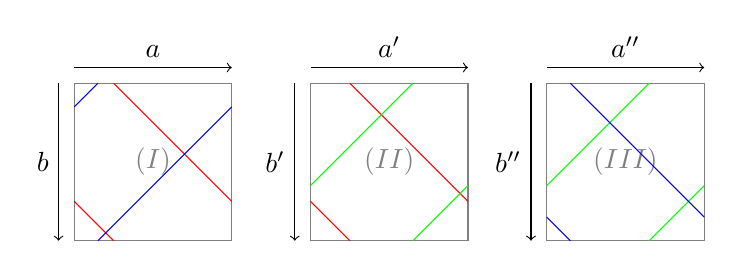
\begin{tikzpicture}
\draw[color=gray]
	[xshift=0cm] (0,0) rectangle (2,2) (1,1) node{$\Lcl(I)$}
	[xshift=3cm] (0,0) rectangle (2,2) (1,1) node{$\Lcl(II)$}
	[xshift=3cm] (0,0) rectangle (2,2) (1,1) node{$\Lcl(III)$};
\draw[->,xshift=0cm] (0,2.2) -- (2,2.2) node[above,midway] {$a$};
\draw[->,xshift=0cm] (-0.2,2) -- (-0.2,0)  node[left,midway] {$b$};
\draw[->,xshift=3cm] (0,2.2) -- (2,2.2) node[above,midway] {$a'$};
\draw[->,xshift=3cm] (-0.2,2) -- (-0.2,0)  node[left,midway] {$b'$};
\draw[->,xshift=6cm] (0,2.2) -- (2,2.2) node[above,midway] {$a''$};
\draw[->,xshift=6cm] (-0.2,2) -- (-0.2,0)  node[left,midway] {$b''$};
\draw[color=red]
	[xshift=0cm] (0.5,0) -- (0,0.5) (0.5,2) -- (2,0.5)
	[xshift=3cm] (0.5,0) -- (0,0.5) (0.5,2) -- (2,0.5);
\draw[color=green]
	[xshift=3cm] (1.3,0) -- (2,0.7) (0,0.7) -- (1.3,2)
	[xshift=3cm] (1.3,0) -- (2,0.7) (0,0.7) -- (1.3,2);
\draw[color=blue]
	[xshift=0cm] (0,1.7) -- (0.3,2) (0.3,0) -- (2,1.7)
	[xshift=6cm,yscale=-1,yshift=-2cm]
		(0,1.7) -- (0.3,2) (0.3,0) -- (2,1.7);
\end{tikzpicture}
\caption{Schnitte zwischen verschiedenen Klassen der regulären Geraden}\label{fig:reg}
\end{figure}

\paragraph{Symmetrien}
% Betrachtung der regulären Situation

\section{Geistergeraden}
\paragraph{Konfiguration}
\paragraph{Symmetrien}
% Betrachtung der irregulären Situation